\documentclass[12pt]{article}
\usepackage{amssymb}
\usepackage{pgfplots}
\pgfplotsset{compat=1.18}
\usepackage{pgfplotstable}
\usepackage{caption}
\usepackage{geometry}
\usepackage{graphicx}
\usepackage{wrapfig}
\usepackage{amsmath}
\usepackage{lipsum}
\usepackage{caption}
\usepackage{ulem}
\usepackage{xcolor}
\usepackage{tikz}
\usetikzlibrary{arrows.meta, positioning, shapes}

\usepackage{sectsty}
\sectionfont{\color{sectionColor}}       % Color for \section
\subsectionfont{\color{subsectionColor}}


\definecolor{titleColor}{HTML}{800000}        % Maroon
\definecolor{sectionColor}{HTML}{4682B4}      % SteelBlue
\definecolor{textHighlight}{HTML}{DAA520}     % Goldenrod
\definecolor{backgroundColor}{HTML}{F0F8FF}   % AliceBlue
\definecolor{emphasisColor}{HTML}{228B22}     % ForestGreen
\definecolor{subsectionColor}{HTML}{6A5ACD}   % SlateBlue

\begin{document}



\section*{Recovery Outcomes after 3 Months (Monte Carlo)}

\begin{figure}[h!]
\centering
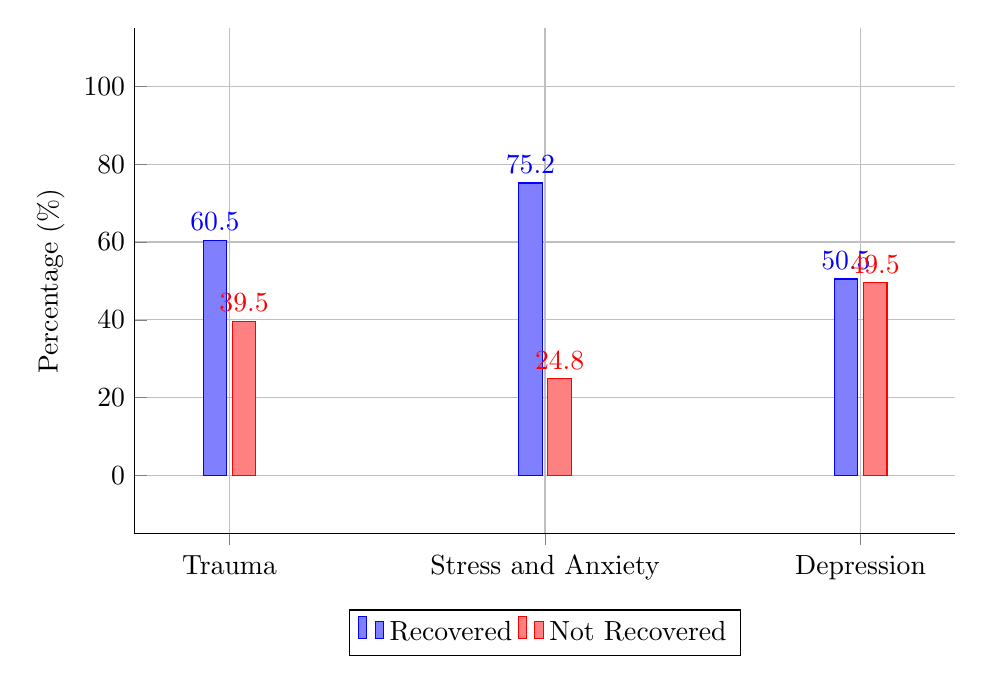
\begin{tikzpicture}
\begin{axis}[
    ybar,
    bar width=0.3cm,
    width=12cm,
    height=8cm,
    enlargelimits=0.15,
    legend style={at={(0.5,-0.15)},
      anchor=north,legend columns=-1},
    ylabel={Percentage (\%)},
    symbolic x coords={Trauma, Stress and Anxiety, Depression},
    xtick=data,
    nodes near coords,
    ymin=0,ymax=100,
    grid=major,
    axis y line*=left,
    axis x line*=bottom
]
\addplot+[style={fill=blue!50}] coordinates {(Trauma,60.5) (Stress and Anxiety,75.2) (Depression,50.5)};
\addplot+[style={fill=red!50}] coordinates {(Trauma,39.5) (Stress and Anxiety,24.8) (Depression,49.5)};
\legend{Recovered, Not Recovered}
\end{axis}
\end{tikzpicture}
\caption{Recovery Outcomes by Condition (Monte Carlo Simulation)}
\end{figure}

\end{document}

